\section{Regelungen}
\subsection{Glieder}

	\begin{tabular}{|l|l|l|l|l|l|}
    	\hline
    	\textbf{Benennung}	&\textbf{Funktion}	&\textbf{UTF}	& \textbf{Sprungantw.}	
    		&\textbf{Verlauf Sprungantw.}	&\textbf{Symbol}\\
    	\hline
    	\hline
    	\textbf{P-Glied} & $y(t)=K u(t)$	& K & K
    	&\begin{minipage}{2.4cm}
         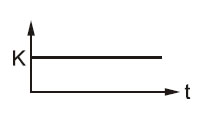
\includegraphics[width=2.4cm]{./bilder/verlaufP.jpg}
         \end{minipage}
    	&\begin{minipage}{2.4cm}
         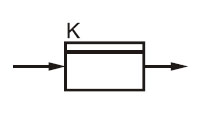
\includegraphics[width=2.4cm]{./bilder/p-Glied.jpg}
         \end{minipage}\\
    	\hline
    	\textbf{I-Glied} &
    	\parbox{3cm}{$\dot{y}= K u(t)$\\
    				$y=K\int \limits_0^t u(t) dt$\\}
    				&$\dfrac{K}{s}$
    	&Kt
    	&\begin{minipage}{2.4cm}
         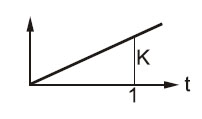
\includegraphics[width=2.4cm]{./bilder/verlaufI.jpg}
         \end{minipage}
    	&\begin{minipage}{2.4cm}
         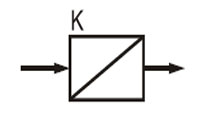
\includegraphics[width=2.4cm]{./bilder/I-Glied.jpg}
         \end{minipage}\\
    	\hline
    	
    	\textbf{Totzeit-Glied}	
    	&$y(t)=\begin{cases} 0 & t < T_t \\u(t-T_t) & t \geq T_t \end{cases}$	&$e^{-T_t s}$	&$K \cdot 1(t-T_t)$
    	&\begin{minipage}{2.4cm}
         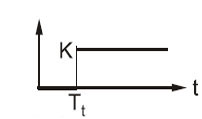
\includegraphics[width=2.4cm]{./bilder/verlaufTt.jpg}\\
        \end{minipage}
    	&\begin{minipage}{2.4cm}
         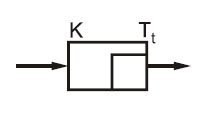
\includegraphics[width=2.4cm]{./bilder/Tt-Glied.jpg}
         \end{minipage}\\
		\hline
		
    	\begin{minipage}{2cm}
			\textbf{PT$_1$-Glied}\\      
         \end{minipage}
		 & 		 
		 \parbox{3cm}{$T\dot{y}+y=K u(t)$\\\\
		 $T = \dfrac{1}{K_i \cdot K_p}$\\
		 $K = \dfrac{1}{K_p}$}	 
		 
		 & $\dfrac{K}{1+Ts}$
    	 & $AK(1-e^{-\frac{t}{T}})+y(0)e^{\frac{t}{T}}$
    	 & \begin{minipage}{2.4cm}
         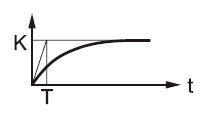
\includegraphics[width=2.3cm]{./bilder/verlaufPT1.jpg}
         \end{minipage}
    	& \begin{minipage}{2.4cm}
         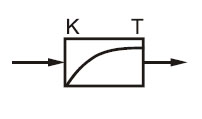
\includegraphics[width=2.3cm]{./bilder/Pt1-Glied.jpg}
         \end{minipage}\\
    	\hline
    \end{tabular}
		
		\begin{minipage}{10cm}
				PT$_1$-Glied mit Grundelementen:\\
			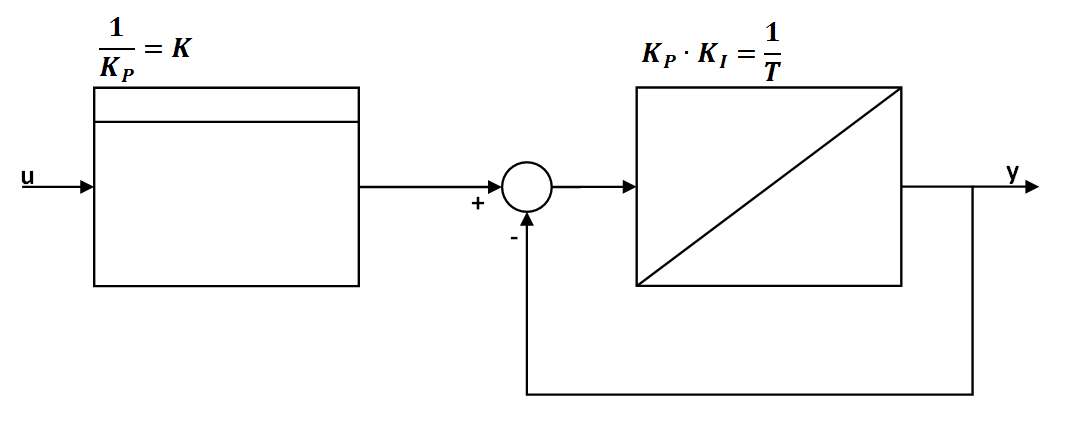
\includegraphics[width=10cm]{./bilder/PT1_2.png}
		\end{minipage}
		\begin{minipage}{8cm}
			$K$: Verstärkung\\
			$T$: Zeitkonstante
		\end{minipage}

    \begin{multicols}{3}
    \textbf{P-Glied (nicht inv. Op-Amp)} \\
    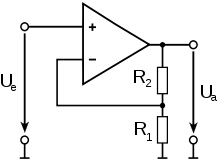
\includegraphics[height=2.5cm]{./bilder/OP-Amp.png} \\
    $K = 1 + \frac{R_2}{R_1}$ 
    \columnbreak

	\textbf{P-Glied (inv. Op-Amp)} \\ 
	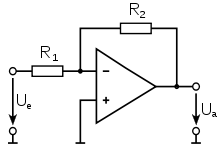
\includegraphics[height=2.5cm]{./bilder/OP-InvAmp.png} \\
	$K=-\frac{R_2}{R_1}$
    \columnbreak
        
    \textbf{I-Glied} \\ 
    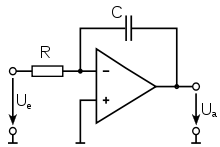
\includegraphics[height=2.5cm]{./bilder/OP-Integrator.png}\\
    $K = - \frac{1}{R \cdot C}$
    \end{multicols}

	\subsection{Stetigähnliche Regler}
		\subsubsection{Rückkopplung des Reglers}
		\begin{minipage}{9cm}
		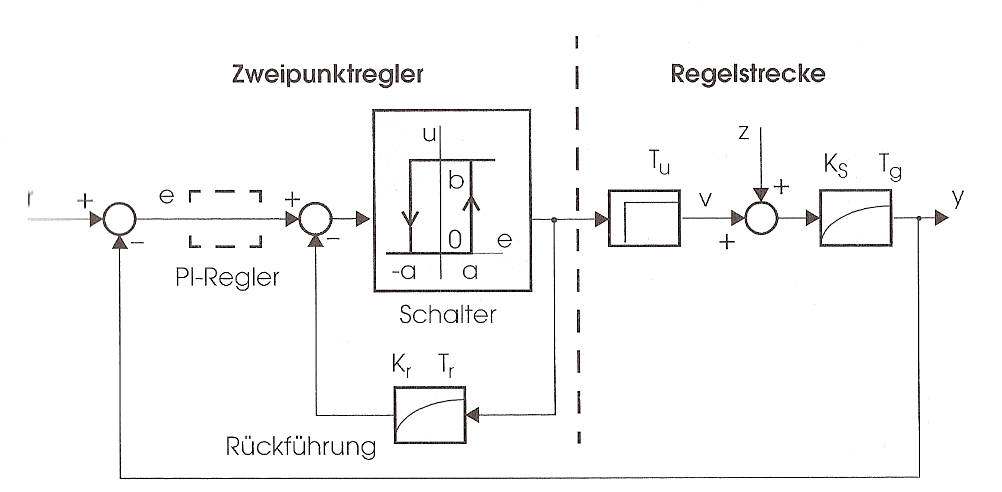
\includegraphics[width=8.5cm]{./bilder/ZweipunktreglerMitRueckfuehrung.jpg}
        \end{minipage}
		\begin{minipage}{7.5cm}
        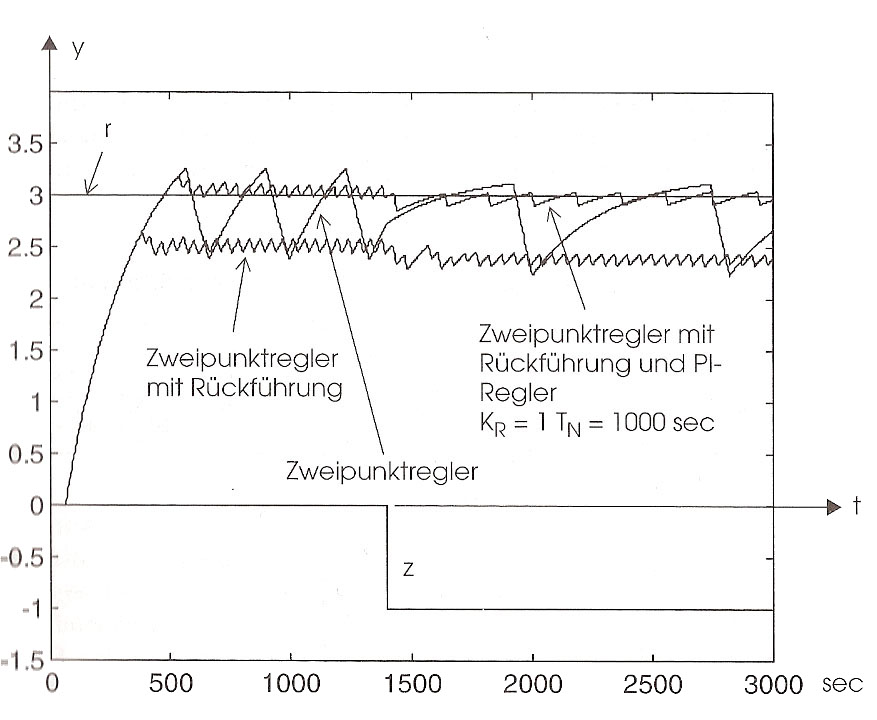
\includegraphics[width=7cm]{./bilder/ZweipunktreglerMitRueckfuehrung_dia.jpg}
        \end{minipage}\\
		Die Rückkopplung mit einem $PT_1$-Glied über dem Zweipunkteregler bewirkt
		einen bedeutend kleineren Rippel. Leider ist der Mittelwert noch unterhalb des
		Sollwertes. Mithilfe eines PI-Reglers vor dem Zweipunkteregler, kann der IST-Wert
		angehoben werden.
	
	\subsubsection{Dreipunktregler}
		\begin{minipage}{9cm}
		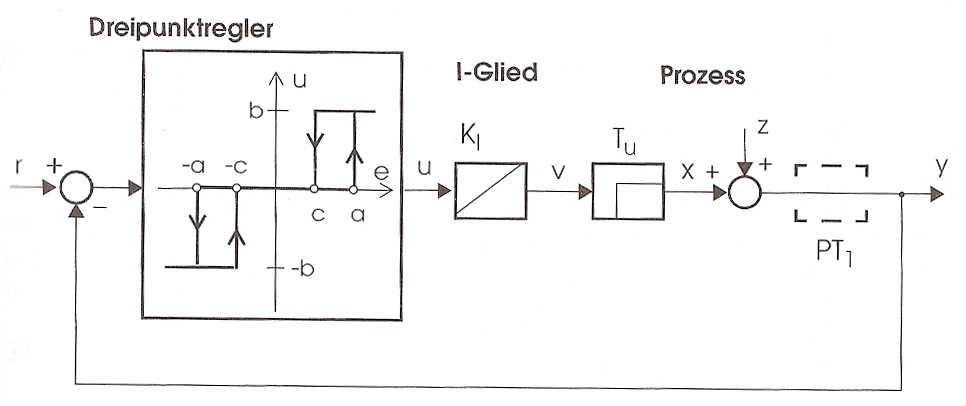
\includegraphics[width=9cm]{./bilder/Dreipunktregler.jpg}
        \end{minipage}
		\begin{minipage}{7.5cm}
        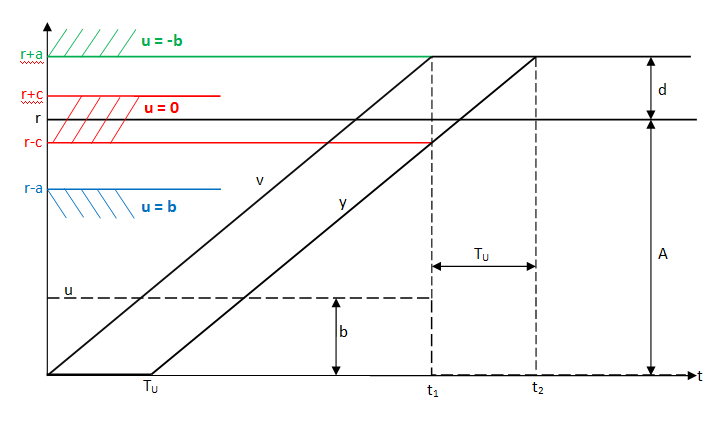
\includegraphics[width=7.5cm]{./bilder/Dreipunkteregler.png}
        \end{minipage}\\
		gewünschtes $\Delta y = c \rightarrow c = K_I \cdot T_u \cdot b$\\
		Falls mit PT$_1$-Glied $\rightarrow c = K_I \cdot K_s \cdot b (T_u + T_G)$
		
		
	\subsubsection{Zweipunktregler}
		\begin{minipage}{3cm}
 		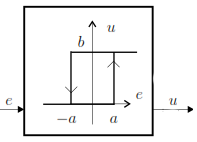
\includegraphics[height=3cm]{./bilder/Zweipunkteregler.png}
        \end{minipage}
		\begin{minipage}{15cm}
        Ein Zweipunktregler ist ein unstetig arbeitender Regler mit zwei
        Ausgangszuständen. Je nachdem, ob der Istwert über oder unter dem
        Sollwert liegt, wird der erste oder der zweite Ausgangszustand
        eingenommen.\\
				$\Delta y = a_2 - a_1$
        \end{minipage}

		\textbf{Beispiele von Zweipunktereglerschaltungen:}\\
		\begin{minipage}{9cm}
			\vspace{.5cm}        
	 		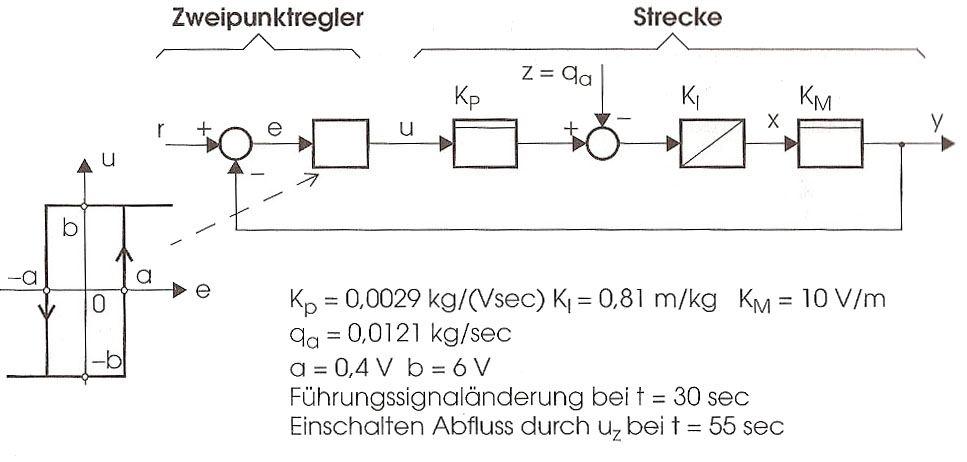
\includegraphics[width=9cm]{./bilder/Zweipunktregler-b+b2.jpg}\\
			Die Anstiegszeit beträgt nach dem Einschwingvorgang:\\
			$t_{ein}=\frac{2a}{(b K_p - q_a)K_i K_m}$ \\ \\
			Die Abfallszeit beträgt nach dem Einschwingvorgang:\\
			$t_{aus}=\frac{2a}{(b K_p + q_a)K_i K_m}$\\
    \end{minipage}
		\begin{minipage}{9cm}
			\vspace{.5cm}        
			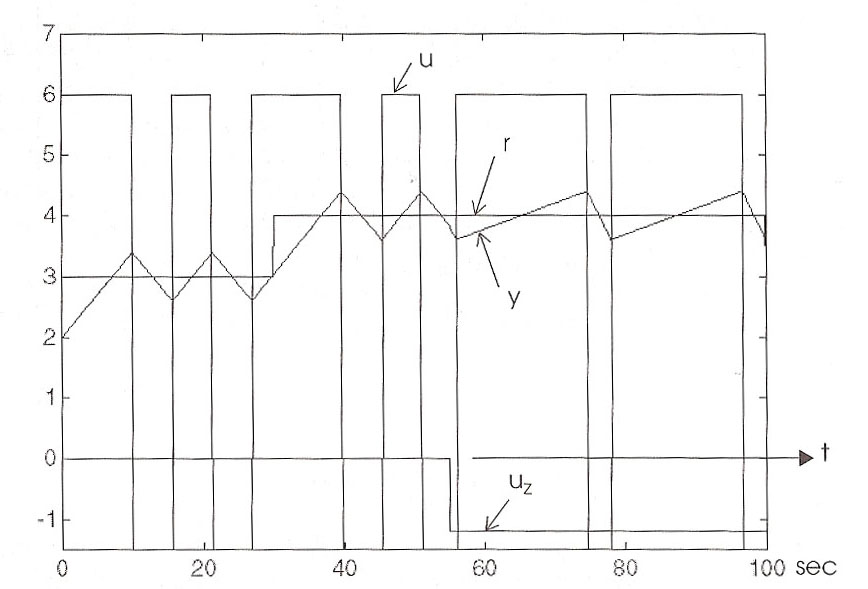
\includegraphics[width=9cm]{./bilder/Zweipunktregler-b+b_dia.jpg}
        \end{minipage}\\
		Einfüllen mit Abfluss: $y = y_0 + K_M \cdot K_I(K_p \cdot b - Q_a)(t-t_0); \qquad$ 
		Abfluss: $y=y_1 + K_M \cdot K_I(K_p(-b) - Q_a)(t-t_0)$
	\vspace{.5cm}
	\hrule
	\vspace{.5cm}
		\begin{minipage}{9cm}
 		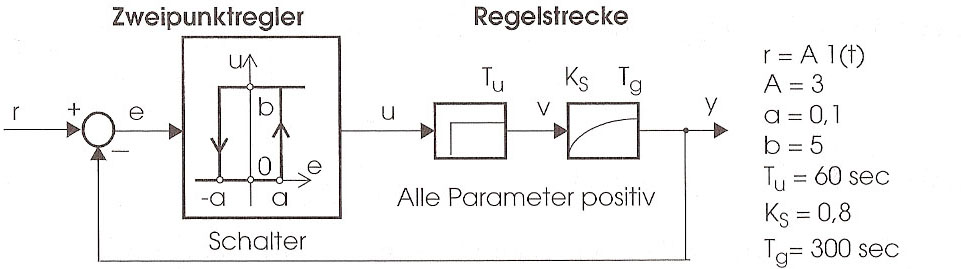
\includegraphics[width=9cm]{./bilder/ZweipunktreglerTotglied2.jpg}\\
			Die Anstiegszeit beträgt nach dem Einschwingvorgang:
			$t_{ein}$=$T_g\ln(\frac{e^{-\frac{T_u}{T_g}}(A-a)-b K_s}{A+a-b K_s})+T_u$\\ \\
			Die Abfallszeit beträgt nach dem Einschwingvorgang:
			$t_{aus}$=$T_g\ln(\frac{A+a-b
			K_s+\frac{b K_s}{e^{-\frac{T_u}{T_g}}}}{A-a})$\\
        \end{minipage}
		\begin{minipage}{9cm}
		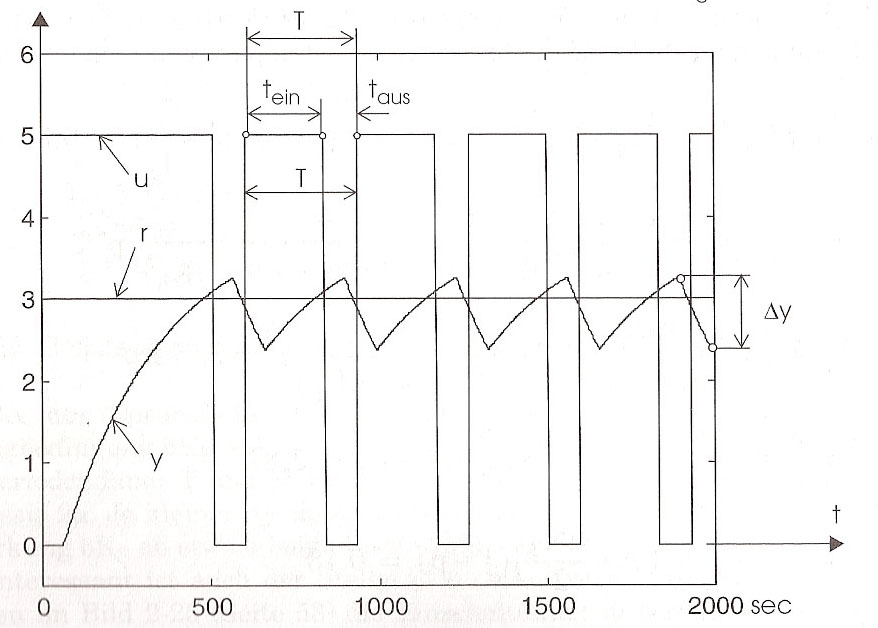
\includegraphics[width=9cm]{./bilder/ZweipunktreglerTotglied_dia.jpg}			
        \end{minipage}
	
	$\Delta y = b\cdot K_s - e^{-\frac{T_u}{T_G}}(b\cdot K_s - 2a); \qquad$
	$y_m = \frac{y_{min}+y_{max}}{2}=e^{-\frac{T_u}{T_G}}\cdot A + \frac{b\cdot K_s}{2}(1-e^{-\frac{T_u}{T_G}}$

	\subsection{Stationäre Signale}
	Für den stationären Fall gelten folgende Bedingungen:
	\begin{itemize}
    	\item \textbf{Fehlersignale} werden jeweils als \textbf{Null} angenommen.
    	\item \textbf{Integratoren} haben am \textbf{Eingang Null}.
    	\item \textbf{Integratoren} haben am \textbf{Ausgang} einen \textbf{beliebigen Wert}.
    	\item \textbf{Totzeitglieder} werden kurzgeschlossen.
    	\item \textbf{PT$_1$-Glieder} wirken als \textbf{P-Glieder} mit $K_P = K_{PT_1}$ behandelt.
  	\end{itemize}